\documentclass[11pt,a4paper]{article}
\usepackage{amsmath}
\usepackage{hyperref}
\usepackage{fullpage}
\usepackage{graphicx}
\usepackage{titling}
\usepackage{titlesec}
\usepackage{enumitem}

% Change heading fonts
\renewcommand{\maketitlehooka}{\sffamily}
\titleformat*{\section}{\Large\bfseries\sffamily}
\titleformat*{\subsection}{\Large\sffamily}
\titleformat*{\subsubsection}{\large\sffamily}

% Put lines under figure captions
\usepackage{caption}
\DeclareCaptionFormat{myformat}{#1#2#3\hrulefill}
\captionsetup[table]{format=myformat}
\captionsetup[figure]{format=myformat}

\begin{document}

\title{Helios \texttt{corefit} data product user guide}
\author{David Stansby \\
\href{mailto:david.stansby14@imperial.ac.uk}{david.stansby14@imperial.ac.uk}}
\maketitle

%%%%
\section{Introduction}
This document describes the Helios \texttt{corefit} data product. This is a new data set which contains estimates of number density, velocity, and temperatures of the proton core population in the solar wind created from systematic fitting of all the original Helios 3D distribution functions.

%%%%
\section{Data availability and documentation}
The data set is freely available at \url{ftp://apollo.ssl.berkeley.edu/pub/helios-data/E1_experiment/New_proton_corefit_data_2017/}. If you do use any of the data in a publication, I would be grateful if you could let me know by emailing \href{mailto:david.stansby14@imperial.ac.uk}{david.stansby14@imperial.ac.uk}.
\newline
\newline
Data are split by probe, year, and day of year. The data are available as either \emph{cdf} or ascii \emph{csv} files with data for each day contained in a single file. Table \ref{tab:variables} summarises the variables present in the data product.
\newline
\newline
The original 3D ion distribution function data are available on the Helios archive FTP server at \url{ftp://apollo.ssl.berkeley.edu/pub/helios-data/E1_experiment/helios_raw/}. Detailed information about the plasma instrumentation can be found at \url{ftp://apollo.ssl.berkeley.edu/pub/helios-data/E1_experiment}. The source code used to read in and fit the distribution functions is available at PUT SOURCE CODE DOI HERE. This code can be used to reproduce the dataset from the original distribution function files.

\begin{table}
	\centering
	\begin{tabular}{| c | c | c | c |}
		\hline
		Parameter 					& Parameter label	& Units			& Note 				\\ \hline \hline \hline
		Time						 	& Time			& 				& 			\\ \hline
		Fitting status					& status			& 				& a	\\ \hline
		Instrument		 			& Instrument		& 				& b	\\ \hline
		Magnetic field instrument			& B instrument		&				& c	\\ \hline \hline
		Proton number density 			& n\_p			& $cm^{-3}$		&	\\ \hline
		Proton $x$ velocity		 		& vp\_x			& $km\cdot s^{-1}$	& \\ \hline
		Proton $y$ velocity		 		& vp\_y			& $km\cdot s^{-1}$	& \\ \hline
		Proton $z$ velocity		 		& vp\_z			& $km\cdot s^{-1}$	&\\ \hline
		Proton perpendicular thermal speed 	& vth\_p\_perp		& $km\cdot s^{-1}$	&\\ \hline
		Proton parallel thermal speed 		& vth\_p\_par		& $km\cdot s^{-1}$	&\\ \hline
		Proton perpendicular temperature	& Tp\_perp		& Kelvin			&	\\ \hline
		Proton parallel temperature	 	& Tp\_par			& Kelvin			&	\\ \hline \hline
		$B_{x}$						& Bx				& nT				& 	\\ \hline
		$B_{y}$						& By				& nT				& 	\\ \hline
		$B_{z}$						& Bz				& nT				& 	\\ \hline
		Magnetic field standard deviation	& sigma B			& nT				& d	\\ \hline \hline
		Sun-spacecraft distance			& r\_sun			& AU				&\\ \hline
		Carrington longitude				& clong			& Degrees		&	\\ \hline
		Carrington latitude				& clat			& Degrees		&	\\ \hline
		Carrington rotation number		& carrot			&				&	\\ \hline
		Spacecraft-Earth angle			& earth\_he\_angle	& Degrees		&	\\ \hline
	\end{tabular}
	\caption{Description of variables present in the \texttt{core\_fit} data product.}	
	\label{tab:variables}
	\small
	\begin{enumerate}[label=\alph*.]
		\item Fitting status flags take the following values: 1: successful fit; 2: successful fit, magnetic field varies too much for reliable number densities and temperatures; 3: successful fit, no magnetic field data available; 4: failed fit
		\item Ion instrument flags take the following values: 1: I1a ion instrument data;  2: I3 ion instrument data
		\item Magnetic field instrument flags take the following values: 1: E3 magnetometer data used;  2: E2 magnetometer data used
		\item Magnetic field standard deviation is calculated as $\sqrt{\sigma^{2}_{Bx} + \sigma^{2}_{By} + \sigma^{2}_{Bz}}$, with individual standard deviations taken over the interval that the ion distribution function was measured
	\end{enumerate}
\end{table}

\newpage
%%%%
\section{Fitting method}
The parameters in the \texttt{corefit} dataset were generated by fitting bi-Maxwellian functions to the original 3D ion distribution functions. The distributions contain contributions from both protons and alpha particles. Because they are well separated in energy, it is easy to fit a distribution to just the protons. Each distribution was fitted using the following process:
\begin{enumerate}
	\item If magnetic field data was available, an average magnetic field was calculated from values taken whilst the distribution function was measured. The distribution function was then rotated into the field aligned frame.
	\item A 3D bi-Maxwellian fit was done of the following form (fit parameters are underlined):
	\begin{equation}
		f_{fit} \left ( v_{\parallel}, v_{\perp 1}, v_{\perp 2} \right ) = \underline{A} \cdot \exp - \left \{ \left ( \frac{v_{\parallel} - \underline{u}_{\parallel}}{\underline{w}_{\parallel}} \right )^{2} + \left ( \frac{v_{\perp 1} - \underline{u}_{\perp 1}}{\underline{w}_{\perp}} \right )^{2} + \left ( \frac{v_{\perp 2} - \underline{u}_{\perp 2}}{\underline{w}_{\perp}} \right )^{2} \right \}
	\end{equation}
	The 6 fit parameters are amplitude ($\underline{A}$), 3 velocities ($\underline{u}_{\parallel}$, $\underline{u}_{\perp 1}$, $\underline{u}_{\perp 2}$), and 2 thermal speeds ($\underline{w}_{\perp}$, $\underline{w}_{\parallel}$). The fit was done using least squares minimisation of the residuals calculated from $\left (f_{data} - f_{fit}\right )$.
	\item The number density was calculated from
	\begin{equation}
		n = \underline{A} \cdot \pi^{3/2}\underline{w}_{\perp}\underline{w}_{\perp}\underline{w}_{\parallel}
	\end{equation}
	and two temperatures from
	\begin{equation}
		T_{\perp / \parallel} = \frac{m_{p}\underline{w}_{\perp / \parallel}^{2}}{2k_{B}}
	\end{equation}
\end{enumerate}
If no magnetic field was available in step 1, steps 2 and 3 still took place, but the thermal speeds and subsequently the number density were ignored. If the magnetic field varies too much during the 32 seconds needed to measure a full distribution the number density and temperatures are unreliable and were thus also ignored.
\newline
\newline
Table \ref{tab:variable availability} summarises which variables are available in each case.
\begin{table}
	\centering
	\begin{tabular}{ c | c | c | c | c}
									& $\mathbf{B}$ available	& $\mathbf{B}$ varies too much	& $\mathbf{B}$ not available	& Failed fits 	\\ \hline
	\texttt{Status} variable value		& 1						& 2							& 3							& 4			\\ \hline
	\texttt{B\_instrument} variable value	& 1 or 2					& -1							& -1							& -1			\\ \hline			
	Number of points 					& 1,869,275				& 34,759							& 192,677					& 119,484	\\ \hline		
	\% points						& 84.3\%					& 1.6\%							& 8.7\%						& 5.4\%		\\ \hline \hline
	Number density					& x						&							&							&			\\ 
	Velocity							& x						& x							& x							&			\\ 
	Temperatures						& x						&							&							&			\\ 
	Magnetic field					& x						&							&							&			\\
	\end{tabular}
	\caption{Summary of which fitted parameters are available depending on magnetic field availability}
	\label{tab:variable availability}
\end{table}
Figure \ref{fig:distribution fit} shows an example of the original distribution function along with the fit.

\begin{figure}
	\centering
	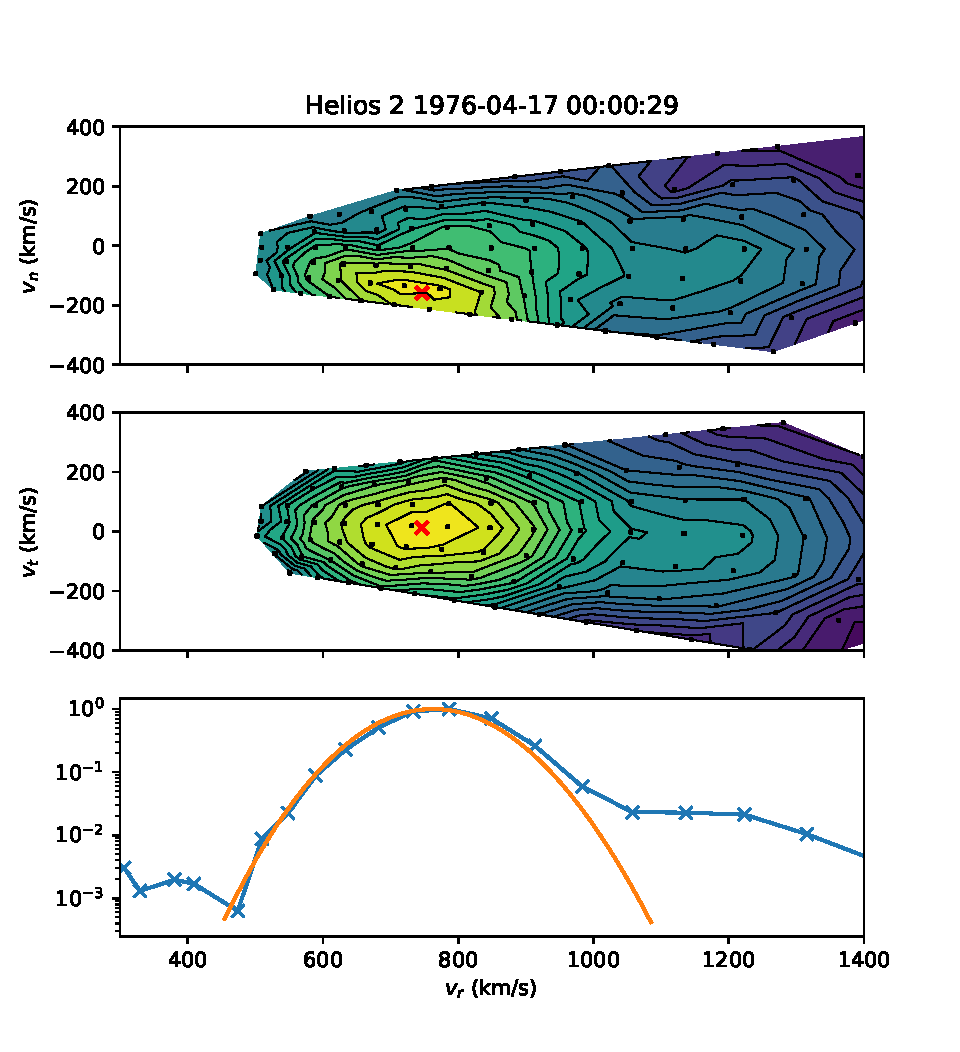
\includegraphics[width=0.7\textwidth]{I3_3D_example}
	\caption{Example of distribution function data and corresponding fit. Top panel shows reduced 2D distribution function in the RN plane of an RTN co-ordinate system. Middle panel shows reduced distribution function in the RT plane. Black dots show positions in velocity space where the distribution function was sampled. Red crosses show the bulk velocity estimate from the fit, which agree well with the data. Bottom panel shows reduced 1D distribution function in blue, with the fit in orange. The fit agrees very well with the data, and is not sensitive to the small proton beam present between 900 to 1100 km/s or the alpha particle population present between 1100 to 1400 km/s.}
	\label{fig:distribution fit}
\end{figure}

%%%%
\section{Differences between \texttt{corefit} and \texttt{merged} data sets}
The \texttt{merged} data set\footnote{Available at \url{ftp://cdaweb.gsfc.nasa.gov/pub/data/helios/helios1/merged/} and \url{ftp://cdaweb.gsfc.nasa.gov/pub/data/helios/helios2/merged/}} is the only other freely available data set with estimates of proton bulk parameters. These parameters were calculated from numerical moments of reduced 1D distribution functions. This means that the \texttt{merged} data does not discriminate between the proton core and proton beam population. Differences between each parameter are as follows:
%%%
\subsection{Number density}
The number density in the \texttt{merged} data set contains contributions from the proton beam, so is systematically higher than the \texttt{corefit} number density. The difference is typically around 10\%, but can be as high as 40\% at times. A time series comparison is shown in figure \ref{fig:density}.
\begin{figure}
	\centering
	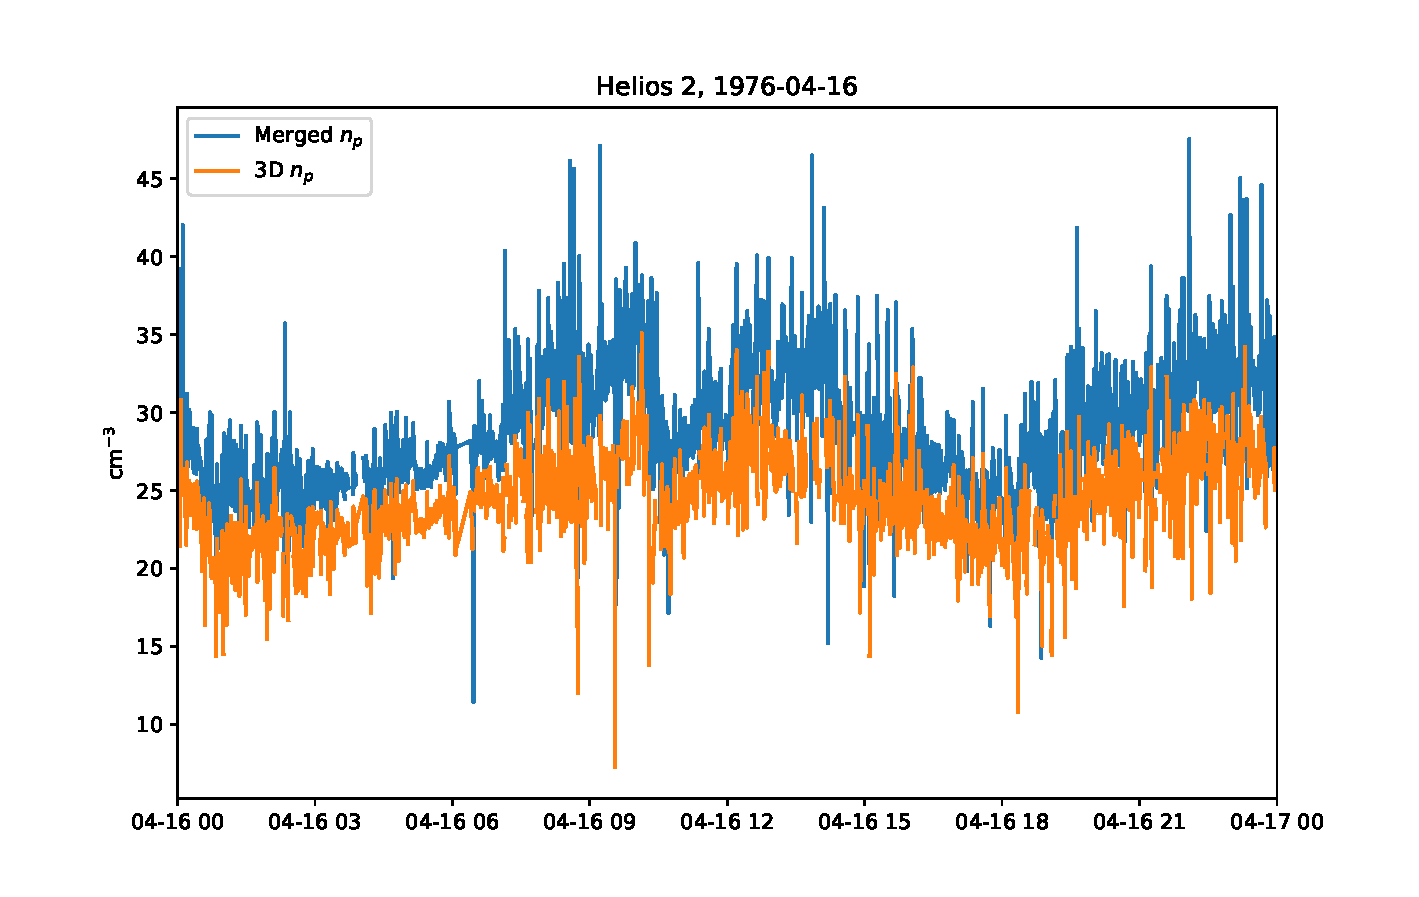
\includegraphics[width=0.8\textwidth]{density_comparison}
	\caption{One day comparison of \texttt{merged} proton number density (blue) and \texttt{corefit} number density (orange). x-axis ticks are every 3 hours with the entire x-axis spanning 1 day, and formatted MM-DD HH.}
	\label{fig:density}
\end{figure}

%%%
\subsection{Velocity}
The radial component of velocity is systematically higher in the \texttt{merged} data set compared to the \texttt{corefit} values, due to the presence of the proton beam. The azimuthal and polar components are not affected by this and the two data sets contain similar values. A time series comparison is shown in figure \ref{fig:velocity}.
\begin{figure}
	\centering
	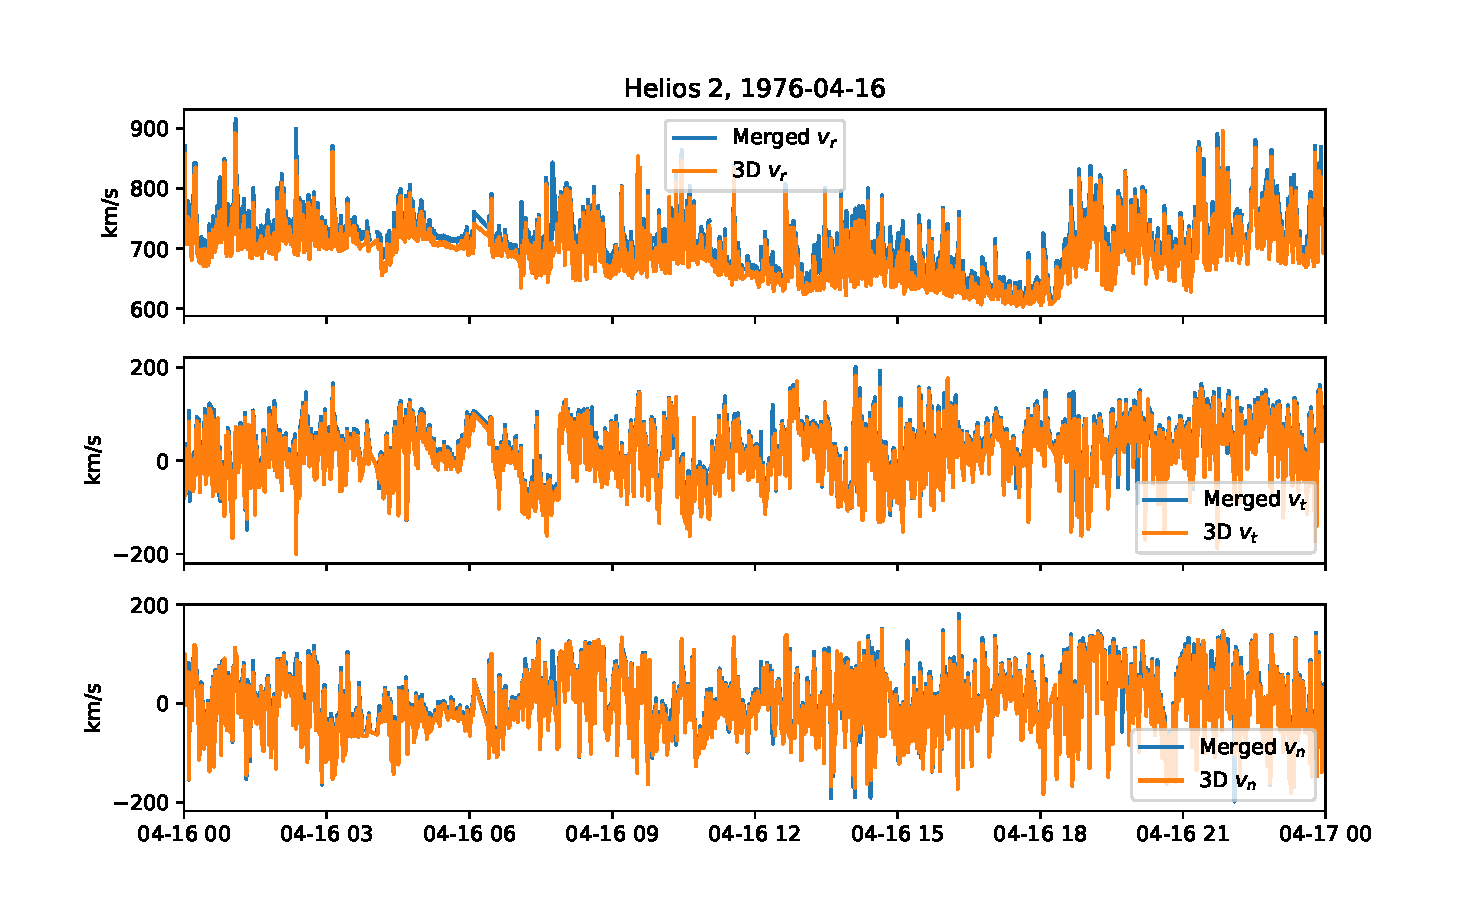
\includegraphics[width=0.8\textwidth]{velocity_comparison}
	\caption{One day comparison of \texttt{merged} proton velocity (blue) and \texttt{corefit} proton velocity (orange) in an RTN co-ordinate system. x-axis ticks are every 3 hours with the entire x-axis spanning 1 day, and formatted MM-DD HH.}
	\label{fig:velocity}
\end{figure}

%%%
\subsection{Temperature}
The \texttt{merged} data set contains only one proton temperature value. This value was calculated from the 1D distribution function which means it contains variable contributions from the true parallel and perpendicular temperatures of the protons. The perpendicular and parallel temperatures in the \texttt{corefit} data set are much more accurate estimates of the temperatures of the proton core. A time series comparison is shown in figure \ref{fig:temperature}.

The total temperature, which can be calculated from the parallel and perpendicular temperatures via.
\begin{equation}
	T = \frac{2T_{\perp} + T_{\parallel}}{3}
\end{equation}
is therefore much more accurate in the \texttt{corefit} data set. The difference between the \texttt{merged} temperature and the \texttt{corefit} temperature can be as big as a factor of 5 (see figure \ref{fig:temperature}, middle panel).

\begin{figure}
	\centering
	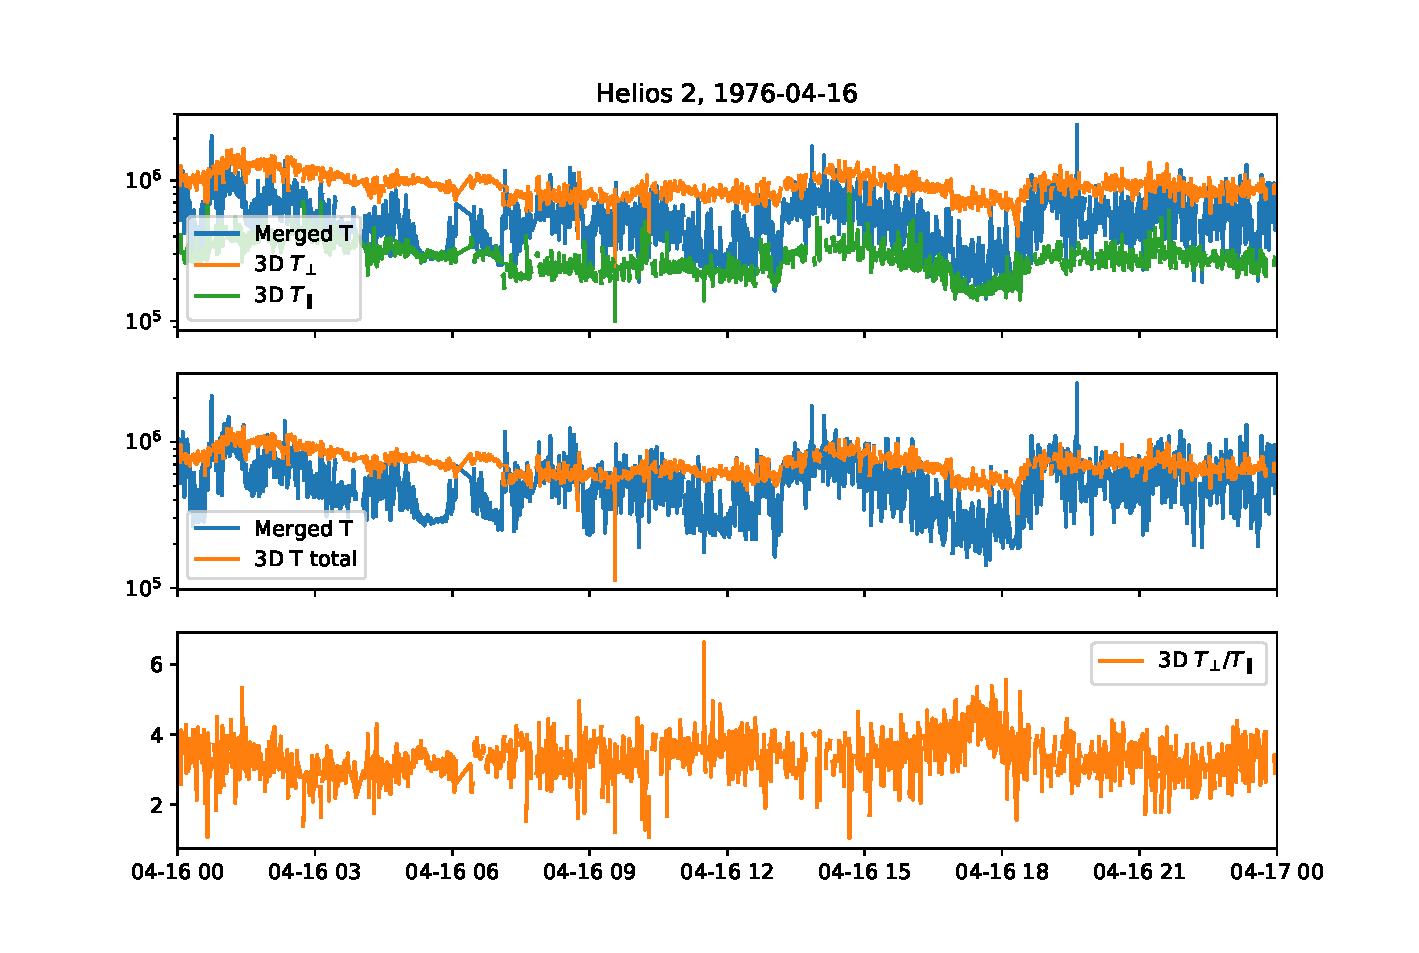
\includegraphics[width=0.8\textwidth]{temperature_comparision}
	\caption{One day comparison of \texttt{merged} proton temperature and \texttt{corefit} proton temperatures. Top panel shows \texttt{merged} proton temperature (blue), \texttt{corefit} perpendicular temperature (orange), and \texttt{corefit} parallel temperature (green). Middle panel shows \texttt{merged} proton temperature (blue) and \texttt{corefit} proton temperature (orange). Bottom panel shows \texttt{corefit} temperature anisotropy (orange). x-axis ticks are every 3 hours with the entire x-axis spanning 1 day, and formatted MM-DD HH.}
	\label{fig:temperature}
\end{figure}

\section{A note on timestamps}
The timestamps in this data set were taken directly from the timestamps given in the filenames of the individual distribution function files. The distributions were originally recorded with a nominal cadence of 40.5 seconds, but it is believed anything after the decimal point in the timestamp has been dropped. This means that the time difference between consecutive time stamps goes like $0, 40, 81, 121, 162...$, whereas the true time differences were $0, 40.5, 81, 121.5, 162...$.
%%%%%
\newpage
\appendix
\section{Acknowledgements}
The work was primarily carried out by David Stansby, in collaboration with Chadi Salem, Lorenzo Matteini, and Tim Horbury. Thanks to Steve Schwartz and Tony Allen for help with cdf files. This work would not have been possible without the invaluable contribution and discussions with the team at the University of Kiel: Lars Berger, Jan Steinhagen, Eckart Marsch, and Robert Wimmer-Schweingruber, as well as Rainer Schwenn. We also acknowledge all the contributions made to the Helios mission and its instruments.

David Stansby is supported by STFC studentship ST/N504336/1. Chadi Salem and work at UC Berkeley is supported by NASA Grant NNX14AQ89G. 
\end{document}